% Transposed content from ieeeaccessA.tex into the IEEE Access template structure
\documentclass{ieeeaccess}
\usepackage{cite}
\usepackage{amsmath,amssymb,amsfonts,amsthm}
\usepackage{algorithm}
\usepackage{algorithmic}
\usepackage{graphicx}
\usepackage{textcomp}
\usepackage{booktabs}
\usepackage{multirow}
\usepackage{tabularx}
\usepackage{array}
\usepackage{url}
\usepackage{bm}
\makeatletter
\AtBeginDocument{\DeclareMathVersion{bold}
\SetSymbolFont{operators}{bold}{T1}{times}{b}{n}
\SetSymbolFont{NewLetters}{bold}{T1}{times}{b}{it}
\SetMathAlphabet{\mathrm}{bold}{T1}{times}{b}{n}
\SetMathAlphabet{\mathit}{bold}{T1}{times}{b}{it}
\SetMathAlphabet{\mathbf}{bold}{T1}{times}{b}{n}
\SetMathAlphabet{\mathtt}{bold}{OT1}{pcr}{b}{n}
\SetSymbolFont{symbols}{bold}{OMS}{cmsy}{b}{n}
\renewcommand\boldmath{\@nomath\boldmath\mathversion{bold}}}
\makeatother

\newcolumntype{Y}{>{\raggedright\arraybackslash}X}
\newtheorem{lemma}{Lemma}
\newtheorem{theorem}{Theorem}
\newtheorem{proposition}{Proposition}
\newtheorem{corollary}{Corollary}

\def\BibTeX{{\rm B\kern-.05em{\sc i\kern-.025em b}\kern-.08em
    T\kern-.1667em\lower.7ex\hbox{E}\kern-.125emX}}

\begin{document}
\history{}
\doi{}
\vol{14}
\year{2026}

\title{Post-Certification Fast Finality in Permissioned Blockchains: A Quantum-Assisted Fail-Closed Framework}
\author{\uppercase{Davy Mateus Nzamba}\authorrefmark{1} and \uppercase{Ricardo Fernandes da Silva}\authorrefmark{2}}

\address[1]{Departamento Academico de Eletrotecnica
Universidade Tecnologica Federal do Parana (UTFPR)
Curitiba, PR, Brazil}
\address[2]{Departamento Academico de Fisica
Universidade Tecnologica Federal do Parana (UTFPR)
Curitiba, PR, Brazil}

\markboth
{Nzamba \headeretal: Post-Certification Fast Finality in Permissioned Blockchains}
{Nzamba \headeretal: Post-Certification Fast Finality in Permissioned Blockchains}

\corresp{Corresponding author: nzamba@alunos.utfpr.edu.br}

\begin{abstract}
This article studies a deliberately narrow problem: whether a quantum-assisted fast path can shorten the post-certification finality interval in permissioned blockchains without enlarging the ledger's safety surface. We introduce Quantum Measurement Consensus (QMC), a fail-closed, post-quorum-certificate ($QC$) service that converts local quantum evidence into a threshold-authenticated common transcript with deterministic ledger semantics and mandatory classical fallback. The main theorem is a safety-preservation result, while the quantitative evaluation is a reproducible deployment-screening study based on phenomenological visibility/fidelity models, policy thresholds, and engineering latency surrogates. The methodology explicitly separates proved properties, assumed cryptographic and BFT guarantees, and modeled operational quantities so that the calibration-to-deployment gap remains visible throughout. Under the baseline surrogate model, pre-provisioned QMC can outperform HotStuff in the bounded post-certification interval for small-to-medium committees, but this conditional advantage is narrow and is rapidly eroded by transcript overhead and on-demand provisioning. The results should therefore be read as a conditional systems-screening framework and architectural thesis, not as hardware-qualified validation or a production-ready quantum consensus claim.
\end{abstract}

\begin{keywords}
Byzantine agreement, fail-closed fast path, GHZ states, HotStuff, permissioned blockchains.
\end{keywords}

\titlepgskip=-15pt
\maketitle

\section{Introduction}
\label{sec:introduction}
\PARstart{I}{n} permissioned blockchains, the most sensitive engineering problem is not always transaction ordering under open membership. In many enterprise, financial, and consortium deployments, the critical question is narrower: a known committee has already validated a candidate block and produced a valid quorum certificate $QC_h$; what remains is the finality step that turns a pre-certified block into an irreversible ledger state. Classical protocols such as Practical Byzantine Fault Tolerance (PBFT), Tendermint, SBFT, and HotStuff solve this problem through authenticated communication, quorum intersection, view change, and explicit fault thresholds \cite{b1,b2,b3,b4,b5,b6}.

Recent quantum-network literature suggests a different resource profile for this final stage. Multipartite entanglement and Greenberger-Horne-Zeilinger (GHZ) measurements can compress committee predicates into coordinated outcomes, potentially reducing latency and making anomalies more detectable. However, the strongest reading of that literature is far more convincing for detectable agreement, liar detection, and specialized subroutines than for replacing the classical control plane of a blockchain outright \cite{b7,b8,b9,b10,b11,b12}.

This article therefore adopts a deliberately narrower formulation: QMC is a fail-closed, post-$QC$ fast-finality service invoked only after the block already carries a valid classical quorum certificate. The quantum layer does not replace quorum formation, ordering, view change, or recovery. Its role is binary: either it accelerates \textit{commit} under verified conditions, or it refuses to finalize and returns control to an always-live classical path.

\subsection{Claim Boundary and Novelty}
The claim boundary is explicit. This article does not propose general quantum consensus; it studies a post-certification finality service for a permissioned ledger whose classical safety proof is already in place. The manuscript does not address transaction ordering, long-horizon throughput, committee reconfiguration, permissionless operation, or quantum consensus in the broad sense. Instead, it isolates the interval between receipt of a candidate block that already carries a valid quorum certificate and the corresponding ledger-level finality acknowledgment.

At its core, the manuscript contributes a ledger-integrated post-certification architecture in which quantum evidence becomes a threshold-authenticated common transcript, coupled to explicit ledger semantics, fail-closed fallback, and regime-based deployment screening. The novelty is not a new safety theorem for Byzantine agreement. Relative to adjacent quantum Byzantine-agreement and detectable-agreement literature, the contribution is the systems combination of five elements:
\begin{enumerate}
    \item post-$QC$ finality isolation, so that the quantum layer is invoked only after classical quorum certification;
    \item threshold-signed common transcript alignment, so that quantum evidence becomes one authenticated ledger input rather than divergent local observations;
    \item tripartite ledger semantics for \textit{commit}, \textit{abort}, and \textit{no-finality};
    \item fail-closed operation with mandatory classical fallback; and
    \item deployment-oriented regime analysis that identifies when the fast path is operationally justified and when it should be disabled.
\end{enumerate}
The main theorem is therefore intentionally a safety-preservation theorem. It proves that QMC does not widen the ledger's safety surface; it does not prove quantum liveness improvement.

The contribution is therefore not a repackaging of quantum Byzantine agreement as blockchain consensus. It is the binding layer that makes a quantum primitive consumable by a ledger after classical certification: transcript authentication, deterministic ledger semantics, explicit fallback, and regime analysis are part of the protocol object rather than external commentary. The novelty is thus architectural and operational rather than foundational: the paper does not introduce a new Byzantine safety theorem, but a disciplined way of inserting a quantum fast path into an already safe classical ledger pipeline.

\subsection{Technical Contributions and Non-Claims}
\label{sec:contributions}
To eliminate interpretive ambiguity, this subsection enumerates exactly what the article contributes and what it does not claim.

\paragraph{Technical Contributions}
\begin{enumerate}
    \item \textbf{Post-$QC$ isolation architecture}: A fail-closed fast-finality service invoked \textit{only after} a candidate block already carries a valid classical quorum certificate. The quantum layer never replaces quorum formation, ordering, view change, or recovery.
    \item \textbf{Threshold-signed common transcript}: A binding mechanism that converts local quantum observations into a single authenticated ledger input, eliminating divergent local interpretations of quantum outcomes.
    \item \textbf{Tripartite ledger semantics}: Explicit \textit{commit}, \textit{abort}, and \textit{no-finality} outcomes with unambiguous ledger-level meaning, rather than treating quantum agreement outputs as uninterpreted binary values.
    \item \textbf{Mandatory classical fallback}: A fail-closed design where any fast-path failure or ambiguity returns control to an always-live classical protocol (HotStuff-compatible).
    \item \textbf{Deployment-oriented regime methodology}: A reproducible screening framework that identifies operational regimes where QMC is justified, marginal, or should be disabled in favor of classical alternatives.
\end{enumerate}

\paragraph{Explicit Non-Claims}
\begin{enumerate}
    \item This article \textbf{does not} propose a general quantum consensus protocol. QMC is strictly a post-certification finality service, not a replacement for classical BFT.
    \item This article \textbf{does not} present hardware-qualified validation. The evaluation uses phenomenological models and engineering surrogates, not measurements from a production QMC prototype.
    \item This article \textbf{does not} prove a universal quantum liveness improvement. The main theorem is safety preservation; liveness of the fast path is conditional on resource quality, timing discipline, and transcript availability.
    \item This article \textbf{does not} apply to permissionless blockchains, dynamic committees larger than $n \approx 16$, or weakly synchronized Internet-scale environments.
    \item This article \textbf{does not} claim that QMC is always superior. The analysis deliberately identifies regimes where HotStuff remains the better engineering choice within scope.
\end{enumerate}
These non-claims are not limitations added after the fact; they define the intended scope of the protocol object from the outset. The paper should therefore be evaluated on whether it provides a sound and useful post-$QC$ fast-finality framework, not on whether it solves general quantum consensus.

The manuscript's contribution is therefore not a replacement for classical BFT, nor a claim of universal quantum superiority. Its contribution is a ledger-integrated binding layer that makes a narrowly scoped quantum primitive consumable after classical certification, together with a reproducible methodology for deciding when that fast path is justified and when it should be disabled. In this sense, the paper is best read as a conservative systems architecture and deployment-screening study for post-$QC$ finality, rather than as a full-stack quantum consensus proposal.


\section{Related Work and Scope}
\subsection{Classical finality in permissioned blockchains}
The classical literature on finality in permissioned systems is robust. PBFT established deterministic safety under authenticated quorums and a three-phase protocol structure \cite{b2}. HotStuff reduced normal-case communication complexity while preserving responsiveness under partial synchrony and is therefore a natural baseline for optimistic finality comparisons \cite{b5}. Work on Hyperledger Fabric, SBFT, Mir-BFT, and blockchain consensus surveys makes clear that the engineering of finality depends on leader behavior, committee topology, ordering policy, and recovery mechanisms \cite{b4,b6,b13,b14,b15,b16}. These protocols solve authenticated finality end to end, but they do not isolate the post-certification interval as an independent optimization target under an auxiliary quantum service.

\subsection{Quantum Byzantine agreement and detectable agreement}
Beginning with the work of Fitzi, Gisin, and Maurer \cite{b7}, followed by Iblisdir and Gisin \cite{b8} and Gaertner \textit{et al.} \cite{b9}, the quantum Byzantine-agreement literature has advanced detectable agreement, liar detection, and related protocols under distinct physical assumptions. More recent works include variants tolerant to any number of dishonest parties \cite{b10}, blockchain-oriented detectable agreement \cite{b11}, integrated-photonics demonstrations \cite{b12}, protocols without entanglement \cite{b17}, and protocols based only on EPR pairs \cite{b18}. Yet these studies rarely couple their primitives to the post-certification finality window of a permissioned ledger.

The reusable part of this literature is the idea that quantum correlations can expose inconsistency or compress a multi-party predicate under strong physical assumptions. The non-reusable part, for the present ledger problem, is equally important: those protocols do not begin from a valid classical quorum certificate, do not define a threshold-signed transcript as the sole ledger input, do not distinguish \textit{abort} from ledger-level \textit{no-finality}, and do not require an always-live classical fallback after a failed quantum attempt. QMC borrows the intuition that quantum evidence can support a fast predicate, but it relocates that predicate inside a classical ledger pipeline rather than treating it as a replacement for the pipeline. What this literature contributes is intuition about correlated predicates and detectability; what it does not contribute is a ledger-consumable, transcript-authenticated post-$QC$ finality mechanism.

\subsection{Multipartite infrastructure and GHZ verification}
Any measurement-based fast path must also be interpreted against the physical literature on the generation, verification, and operation of multipartite resources. Recent studies address optimal Bell/GHZ verification in untrusted quantum networks \cite{b19}, global GHZ creation on quantum processors \cite{b20}, scalable multipartite-entanglement determination \cite{b21}, entanglement distribution in lossy networks \cite{b22}, and larger reconfigurable photonic quantum networks \cite{b23}. These works provide the physical plausibility of the resource layer, but not the ledger semantics, transcript discipline, or fallback logic required by permissioned finality.

\subsection{Why the existing literature does not answer the post-$QC$ finality question}
The gap addressed here is therefore operationally precise: prior work either solves authenticated finality without quantum assistance, or studies quantum agreement without ledger-level post-certification semantics. This manuscript targets the missing bridge between those two domains.

This bridge matters because a permissioned ledger does not merely need parties to observe a quantum outcome. It needs one authenticated object that can be checked, logged, audited, and interpreted identically by all honest replicas at a particular height. The threshold-signed transcript is therefore not a presentation detail; it is the mechanism that turns local quantum observations into a ledger-consumable finality input.

\begin{table*}[!t]
\caption{Positioning of the contribution relative to the state of the art.}
\label{tab:novelty}
\centering
\footnotesize
\renewcommand{\arraystretch}{1.16}
\begin{tabularx}{\textwidth}{p{2.5cm}p{2.5cm}p{2.4cm}p{1.6cm}p{1.5cm}Y}
\toprule
\textbf{Work class} & \textbf{Target problem} & \textbf{Source of safety} & \textbf{Classical fallback} & \textbf{Quantum resource} & \textbf{Gap relative to this article} \\
\midrule
PBFT/HotStuff and variants \cite{b2,b4,b5} & Authenticated BFT finality end to end & Quorum intersection and authentic signatures & Native to the protocol & No & Do not explore a quantum post-$QC$ fast path. \\
Quantum Byzantine agreement / detectable agreement \cite{b7,b8,b9,b10,b11,b12,b17,b18} & Agreement, detectability, or liar detection & Properties of the quantum protocol and communication model & Usually not modeled as a ledger pipeline & Yes & Do not address the narrow post-certification finality window in permissioned blockchains. \\
Multipartite quantum infrastructure \cite{b19,b20,b21,b22,b23} & Resource distribution, verification, and operation & Outside ledger scope & No & Yes & Provide the physical substrate, but not an integrated ledger-level finality semantics. \\
\textbf{This article} & \textbf{Post-$QC$ fast finality in a permissioned ledger} & \textbf{Classical safety only; the quantum layer adds no new safety surface} & \textbf{Mandatory} & \textbf{Verified GHZ multipartite resource} & \textbf{Combines post-$QC$ isolation, threshold-signed transcript alignment, tripartite outputs, fail-closed fallback, and deployment-oriented regime maps.} \\
\bottomrule
\end{tabularx}
\end{table*}

\section{System Model and Assumptions}
\label{sec:model}
We consider a permissioned committee with $n = 3f + 1$ validators and at most $f$ Byzantine participants. Membership is known, signatures are authenticated, and no honest validator signs conflicting blocks at the same block height. After a global stabilization point, the classical network satisfies partial synchrony with a reference delay $\Delta$ \cite{b24,b25}. At height $h$, each validator receives a candidate block $B_h$ together with a valid classical quorum certificate $QC_h$ containing $q = 2f + 1$ signatures on the same block hash.

Each validator first executes local classical validation before invoking the quantum fast path. Define the local readiness bit as
\begin{equation}
\chi_i(h,r)=
\begin{cases}
0, & \text{if all local validation tests pass},\\
1, & \text{otherwise},
\end{cases}
\label{eq:chi}
\end{equation}
so that $\chi_i=0$ means validator $i$ is locally ready to finalize the already pre-certified block during round $r$.

The local tests aggregate verification of $QC_h$, the block body $B_h$, and the expected post-state root. The event of interest for the fast path is
\begin{equation}
E_{h,r} = \bigl(QC_h \text{ valid}\bigr) \wedge \bigl(\chi_i(h,r)=0,\ \forall i \in H\bigr),
\label{eq:event}
\end{equation}
where $H$ denotes the set of honest validators active in round $r$.

\subsection{Adversarial Scope}
The adversary is Byzantine at the validator layer but bounded by the classical threshold $f$. It may delay, omit, reorder, or selectively deliver control-plane messages before the partial-synchrony bound applies; it may corrupt at most $f$ validators; it may degrade quantum-resource quality, perturb local phase behavior, increase timing skew, or cause transcript shares to be delayed or omitted. The adversary is not assumed to break digital signatures, threshold-signature unforgeability, collision resistance of the transcript hash, or the classical quorum-certificate rule that honest validators sign at most one block per height. It also cannot produce two valid classical quorum certificates for conflicting blocks without violating the classical BFT assumptions.

\begin{table}[H]
\caption{Consolidated threat model for the QMC fast path.}
\label{tab:threat}
\centering
\scriptsize
\setlength{\tabcolsep}{3.4pt}
\renewcommand{\arraystretch}{1.12}
\begin{tabularx}{\columnwidth}{p{1.75cm}Yp{1.15cm}}
\toprule
\textbf{Surface} & \textbf{Allowed adversarial action} & \textbf{Effect} \\
\midrule
Classical ledger & Byzantine behavior by at most $f$ validators; message delay under partial synchrony & Safety preserved by quorum intersection; liveness inherited from fallback \\
Quantum resource & Fidelity degradation, parity disturbance, phase inversion, loss & Lower fast-commit probability; \textit{abort} or \textit{no-finality} \\
Timing discipline & Increased skew or coordinated misalignment & Abort-dominant fast-path behavior \\
Transcript delivery & Selective share omission, aggregator delay, invalid transcript emission & Availability loss for QMC; no conflicting commits \\
Out of scope & Signature forgery, hash collision, conflicting valid $QC_h$ values, permissionless membership & Violates base assumptions \\
\bottomrule
\end{tabularx}
\end{table}

\subsection{Timing discipline of the fast path}
The temporal discipline assumed by the fast path is the ability to measure and bound the spread between local acquisition times of the quantum outcome and the associated authenticated evidence. Let $\delta_r$ denote the inter-validator skew measured as the difference between the largest and smallest local timestamps associated with transcript acceptance in round $r$. This model represents managed datacenter or metropolitan-fiber environments, not weakly synchronized Internet-scale deployments. If timestamps diverge beyond $\Delta_{\max}$, the round is not promoted to \textit{commit}; it is classified as \textit{abort} or \textit{no-finality}, depending on the remaining evidence.

\subsection{Threshold-Signed Transcript Service}
To prevent divergent local interpretations of quantum outcomes, the primary realization used in this article is a threshold-signed transcript aggregator. The committee has a threshold public key for transcript certification and each validator holds one signing share. The transcript domain separates ledger height, fast-path round, block hash, and quorum-certificate hash, so a share for one round cannot be replayed as evidence for another round.

The message flow is concrete. After validating $(B_h,QC_h)$ and obtaining the local quantum evidence, validator $i$ sends the aggregator a signed share over
\begin{equation}
m_{i,r}=\left(h,r,\mathrm{hash}(B_h),\mathrm{hash}(QC_h),\widehat{F}_{i,r},t_{i,r},\widehat{\pi}_{i,r}\right).
\label{eq:share}
\end{equation}
The aggregator accepts only well-formed shares whose ledger identifiers match the candidate block. It canonicalizes the round by deriving $\widehat{F}_r$ from the accepted fidelity evidence, $\widehat{\delta}_r=\max_i t_{i,r}-\min_i t_{i,r}$ from the accepted timestamps, and $\widehat{\pi}_r$ from the accepted parity evidence. Once at least $q=2f+1$ compatible shares are available, the aggregator combines them into a threshold signature over the transcript hash and multicasts the resulting transcript to all validators.

This design adds one upload step, one threshold-combination step, and one multicast step to the post-certification finality interval. In the common case the coordination cost is linear in the committee size: $O(n)$ signed uploads, one threshold-signature combination, and $O(n)$ dissemination messages. The cost of this service is included in the QMC latency surrogates in Section~\ref{sec:method}. If the aggregator is slow, censors shares, observes incompatible evidence, fails to collect $2f+1$ compatible shares before timeout, or emits an invalid threshold signature, honest validators reject the fast path and invoke the classical fallback. Thus the main failure mode is loss of fast-path availability, not a new safety failure.

Operationally, the transcript service is a systems bottleneck. Its latency contribution can be decomposed as
\begin{equation}
T_{TS}=T_{up}+T_{queue}+T_{comb}+T_{cast}+T_{verify},
\label{eq:tts}
\end{equation}
where $T_{up}$ is share upload delay, $T_{queue}$ is scheduler or batching delay at the aggregator, $T_{comb}$ is threshold-signature combination, $T_{cast}$ is dissemination of the completed transcript, and $T_{verify}$ is local verification by validators. This transcript service is not an implementation footnote. It is the key systems bottleneck of the proposal: if its p95 delay, batching behavior, or share-collection latency approaches the available break-even margin, QMC loses its operational rationale even when the quantum resource itself remains acceptable. The baseline latency model folds these terms into $T_{QMC}$, while $p_{cp}$ captures residual timeout, share-collection failure, or transcript unavailability. If the fast path is invoked at rate $\lambda$ and the transcript service has mean service time $s$, then sustained operation requires traffic intensity $\rho=\lambda s<1$; as $\rho$ approaches one, queueing delay dominates and the service should be disabled because the quantum path no longer provides a useful finality-interval advantage.

For this reason, the transcript layer should be interpreted as part of the protocol object rather than as auxiliary middleware.

Selective omission is treated as an availability attack. A censoring aggregator can exclude honest shares, wait for a more favorable subset, or simply fail to publish a transcript before timeout. It cannot make omitted shares support a conflicting accepted transcript without a threshold-signature break, but it can move probability mass from \textit{commit} to \textit{no-finality} or \textit{abort}. Deployments can reduce this centrality by rotating the aggregator per height, running two or more accountable aggregators in parallel and accepting the first valid threshold transcript, or replacing the single collector with a replicated transcript service that gossips shares and deterministically constructs the same transcript. These variants raise dissemination cost toward $O(n^2)$ in the worst case and may erode the latency advantage, but they trade a single queueing point for better fast-path availability.

The threshold transcript does not reopen safety vulnerabilities because a valid transcript signature requires $2f+1$ shares. Any two such share sets intersect in at least one honest validator, and honest validators sign at most one canonical transcript share for a fixed $(h,r,\mathrm{hash}(B_h),\mathrm{hash}(QC_h))$ domain. Aggregator equivocation can therefore be detected unless the threshold-signature scheme or the classical quorum assumptions fail. Accordingly, the practical value of QMC depends not only on quantum-resource quality but also on transcript-service discipline under bounded load.

\section{Protocol Semantics and Architecture}
\label{sec:semantics}
Figure~\ref{fig:architecture} summarizes the architecture, and Figure~\ref{fig:sequence} shows the operational sequence from receipt of $(B_h,QC_h)$ to either ledger decision or fallback. Instead of allowing each validator to interpret the measurement outcome locally, QMC lifts fast-path evidence into a common authenticated ledger input. For an ideal committee GHZ state,
\begin{equation}
\lvert GHZ_n \rangle = \frac{\lvert 0 \rangle^{\otimes n} + \lvert 1 \rangle^{\otimes n}}{\sqrt{2}},
\label{eq:ghz}
\end{equation}
each validator applies a local phase encoding
\begin{equation}
U_i(\chi_i)=\exp\!\left(-\frac{i\pi}{2}\chi_i\sigma_z^{(i)}\right),
\label{eq:encoding}
\end{equation}
and the committee measures the parity observable
\begin{equation}
\Pi = \bigotimes_{i=1}^{n}\sigma_x^{(i)}.
\label{eq:parity}
\end{equation}

The authenticated transcript of round $r$ is
\begin{equation}
Tr_r = \left(h, \mathrm{hash}(B_h), QC_h, \widehat{F}_r, \widehat{\delta}_r, \widehat{\pi}_r, \sigma^{TS}_r\right),
\label{eq:transcript}
\end{equation}
where $\widehat{F}_r$ is the verified fidelity estimate, $\widehat{\delta}_r$ is the inter-validator timing spread, $\widehat{\pi}_r \in \{+1,-1\}$ is the observed parity sign, and $\sigma^{TS}_r$ is the threshold signature of the committee shares on the transcript hash.

Ledger-level decision rules are
\begin{subequations}
\label{eq:rules}
\begin{align}
\mathrm{commit}(B_h) \Leftrightarrow {} & \bigl(QC_h \text{ valid}\bigr) \wedge \widehat{F}_r \geq F_{\min} \notag \\
& \wedge \widehat{\delta}_r \leq \Delta_{\max} \wedge \widehat{\pi}_r = +1, \label{eq:commit} \\
\mathrm{abort}(B_h) \Leftrightarrow {} & \widehat{F}_r < F_{\min} \vee \widehat{\delta}_r > \Delta_{\max} \notag \\
& \vee \bigl(Tr_r \text{ absent or unauthenticated}\bigr), \label{eq:abort} \\
\mathrm{nof}(B_h) \Leftrightarrow {} & \neg \mathrm{commit}(B_h) \wedge \neg \mathrm{abort}(B_h). \label{eq:nof}
\end{align}
\end{subequations}

The tripartite semantics is operationally important. \textit{Commit} means immediate and irreversible ledger finalization. \textit{Abort} is a hard stop of the fast path, with immediate classical fallback. \textit{No-finality} is a null output of the fast path and is not itself a conflicting ledger state; it only authorizes a retry or direct return to the classical path, depending on deployment policy.

\begin{figure*}[!t]
\centering
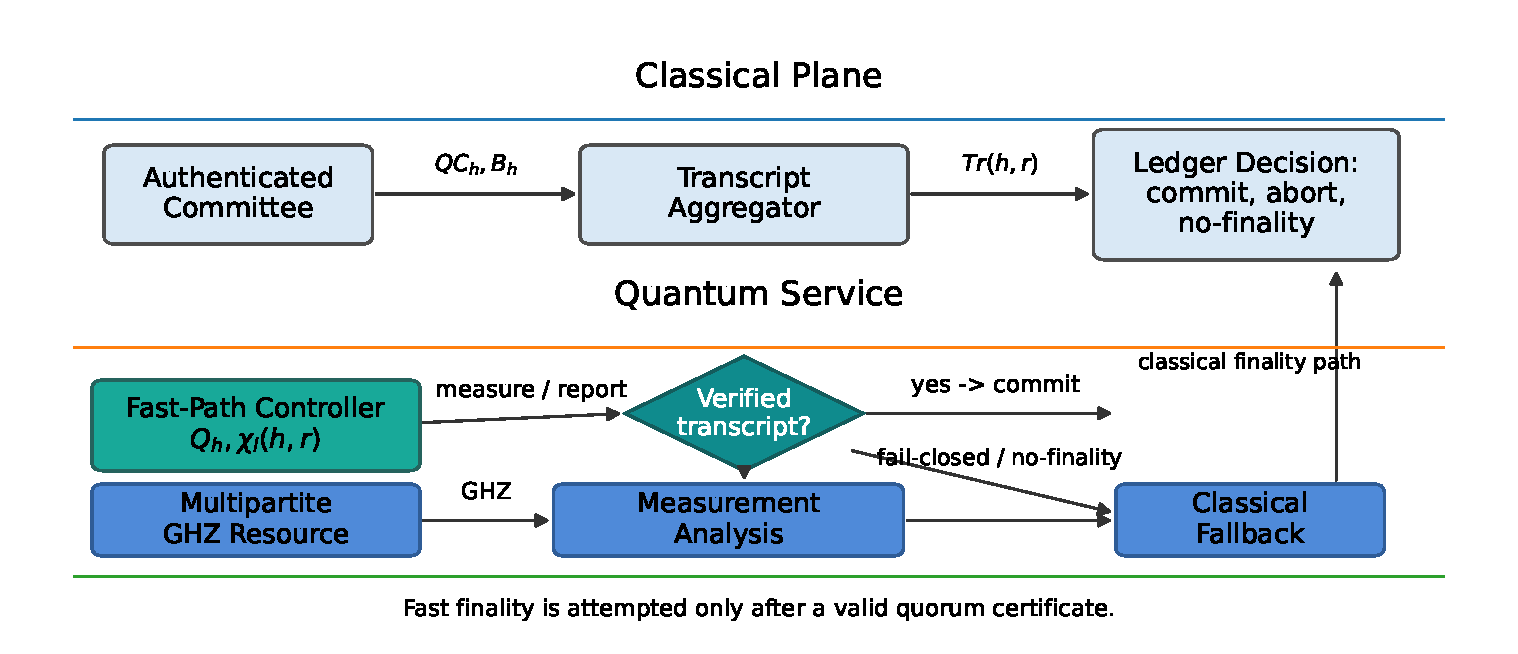
\includegraphics[width=0.96\textwidth]{fig1_architecture.pdf}
\caption{QMC as a post-certification fast-finality service. The quantum plane is activated only after classical pre-certification and never enlarges the safety surface of the ledger; it either accelerates \textit{commit} under verified conditions or hands control back to classical recovery.}
\label{fig:architecture}
\end{figure*}

\begin{figure*}[!t]
\centering
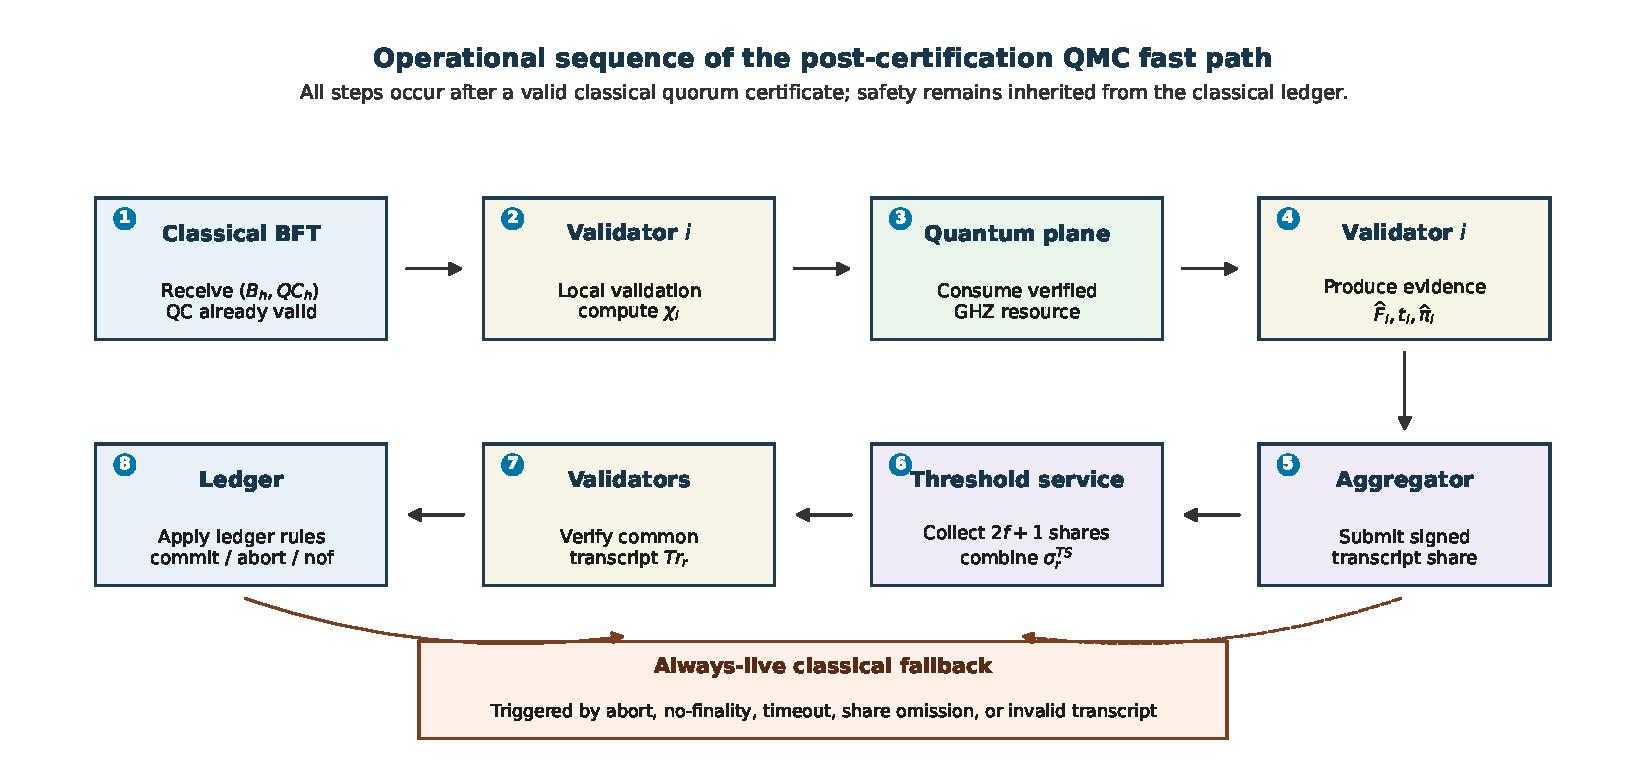
\includegraphics[width=0.98\textwidth]{fig5_sequence.pdf}
\caption{Sequence-style view of one QMC round. The fast path begins only after a valid $(B_h,QC_h)$ pair has been received. Local validation and quantum evidence generation are followed by transcript-share submission, threshold aggregation, transcript verification, ledger-rule application, and immediate fallback on timeout, invalid transcript, \textit{abort}, or \textit{no-finality}.}
\label{fig:sequence}
\end{figure*}

\begin{algorithm}[!t]
\caption{Operational procedure of a QMC round}
\label{alg:qmc}
\begin{algorithmic}[1]
\REQUIRE $h$, $B_h$, $QC_h$, verified multipartite resource, transcript threshold key
\STATE Verify the classical certificate and the hash of $B_h$
\STATE Compute $\chi_i(h,r)$ using~\eqref{eq:chi}
\IF{$\chi_i(h,r)=1$}
    \STATE Refuse the fast path and invoke classical recovery
\ENDIF
\STATE Consume the multipartite resource and obtain $(\widehat{F}_r,\widehat{\delta}_r,\widehat{\pi}_r)$
\STATE Sign one transcript share for the canonical round domain in~\eqref{eq:share}
\STATE Combine at least $2f+1$ compatible shares into $Tr_r$ according to~\eqref{eq:transcript}
\STATE Verify the transcript threshold signature $\sigma^{TS}_r$
\STATE Apply the ledger rules in~\eqref{eq:rules}
\IF{$\mathrm{abort}(B_h)$ or $\mathrm{nof}(B_h)$}
    \STATE Invoke the always-live classical fallback
\ENDIF
\end{algorithmic}
\end{algorithm}

\section{Correctness and Operational Implications}
\label{sec:correctness}
\begin{lemma}[Alignment through a common transcript]
If honest validators apply~\eqref{eq:rules} to the same authenticated transcript $Tr_r$, then they evaluate the same quality, timing, and parity predicates for that round.
\end{lemma}
\begin{proof}
The only logical purpose of $Tr_r$ is to eliminate divergence of local interpretation. If the transcript hash is authenticated and common to all honest validators, then acceptance and rejection decisions become deterministic at ledger level.
\end{proof}

\begin{lemma}[Threshold-transcript non-equivocation]
Assume the threshold-signature scheme is unforgeable and each honest validator signs at most one transcript share for a fixed $(h,r,\mathrm{hash}(B_h),\mathrm{hash}(QC_h))$ domain. Then a Byzantine aggregator cannot make two conflicting transcripts for that domain acceptable to honest validators.
\end{lemma}
\begin{proof}
Each accepted transcript requires at least $2f+1$ valid shares. Two such sets intersect in at least $f+1$ validators, at least one of which is honest. That honest validator signs only one canonical transcript share for the domain, so two conflicting threshold-signed transcripts cannot both be produced unless a signature is forged or an honest-signing rule is violated.
\end{proof}

\begin{theorem}[Safety preservation, not quantum liveness]
Assume at most $f$ Byzantine validators, classical threshold $q=2f+1$, uniqueness of honest signatures per block height, an unforgeable threshold-signed transcript, and application of~\eqref{eq:rules} over the same authenticated transcript. Then two honest validators cannot \textit{commit} conflicting blocks at the same height through QMC.
\end{theorem}
\begin{proof}
Every fast commit requires a valid $QC_h$. In a committee with $n=3f+1$, any two sets of $2f+1$ signatures intersect in at least $f+1$ validators. Since at most $f$ can be Byzantine, at least one signer in the intersection is honest. Honest validators do not sign conflicting blocks at the same height. Therefore, two conflicting quorum certificates cannot both be valid for honest fast commits. The quantum layer can accelerate or refuse finality, but it does not create safety beyond what the classical layer already guarantees.
\end{proof}

\begin{corollary}[No safety amplification]
QMC does not enlarge the safety surface of the ledger; it only accelerates decisions that are already safe under classical quorum intersection when the operational fast-path predicates hold.
\end{corollary}

\begin{proposition}[Null nature of \textit{no-finality}]
\textit{No-finality} is a null output of the fast path and is not a conflicting ledger state. Its operational effect is only to delay finalization or to trigger classical fallback.
\end{proposition}

\begin{proposition}[Fail-closed behavior under transcript and resource degradation]
If an adversary can degrade the quantum resource, the fidelity estimate, timing discipline, or transcript delivery, but cannot forge classical signatures or produce conflicting valid quorum certificates, then the adversary can reduce fast-commit probability and increase the probability of \textit{abort} or \textit{no-finality}, but cannot induce conflicting commits through QMC.
\end{proposition}

The behavior of the transcript service deserves special emphasis. Aggregator delay, selective share omission, or transcript unavailability can suppress the fast path, but they do not create ledger-level safety violations as long as threshold-signature unforgeability and classical quorum assumptions hold. Operationally, this means transcript faults are availability faults for QMC, not safety faults for the underlying ledger.

\begin{proposition}[Conditional fast-path availability]
If a valid $QC_h$ exists, all honest local validation tests pass, a verified quantum resource satisfies $\widehat{F}_r\geq F_{\min}$, timing satisfies $\widehat{\delta}_r\leq\Delta_{\max}$, parity evidence satisfies $\widehat{\pi}_r=+1$, and a valid threshold transcript is delivered before timeout, then honest validators that receive the transcript apply the same \textit{commit} decision for that fast-path round. If any of these operational predicates fails, QMC provides no fast-path liveness guarantee and the protocol invokes classical fallback.
\end{proposition}

This proposition is deliberately conditional. The safety theorem above is deterministic under classical BFT assumptions; the availability proposition depends on resource quality, timing, queueing, and transcript delivery. This distinction is central to the paper's evidentiary structure. Safety is inherited from classical quorum intersection and transcript authenticity, whereas fast-path usefulness is conditional on resource quality, timing discipline, and transcript delivery. The manuscript therefore proves non-amplification of safety claims and evaluates the operational plausibility of latency improvement, rather than proving a universal quantum liveness gain.

If a single attempt has probabilities $(p_c,p_a,p_n)$ for \textit{commit}, \textit{abort}, and \textit{no-finality}, then a second independent attempt after \textit{no-finality} yields the engineering approximation
\begin{equation}
p_c^{(1R)} = p_c + p_n p_c.
\label{eq:retry}
\end{equation}
Equation~\eqref{eq:retry} is not a protocol guarantee; it is a deployment-oriented approximation that indicates when a single retry still materially improves the probability of fast commit.

\section{Evaluation Methodology}
\label{sec:method}
\subsection{Phenomenological visibility model}
To keep the study reproducible and parameter-traceable, the simulation uses the effective visibility
\begin{equation}
V(n,\theta)=e^{-\alpha (n-1)}(1-\varepsilon_s)^n(1-2p_d)^n\exp\!\left[-\left(\frac{\sigma_t}{\tau_0}\right)^2\right],
\label{eq:visibility}
\end{equation}
where $\theta=(\varepsilon_s,p_d,\sigma_t,p_{cp})$ captures state-preparation infidelity, readout/detection error, timing jitter, and residual control-plane failure. The fidelity proxy is
\begin{equation}
F(n,\theta)=\frac{1+V(n,\theta)}{2}.
\label{eq:fidelity}
\end{equation}
The model is not intended to predict a specific hardware platform; it is a system-level instrument for testing how committee size, noise, and orchestration affect the operational credibility of the fast path. The acceptance threshold should therefore be read as a policy knob over verified evidence, not as a claim that one hardware family already satisfies all ledger-facing requirements.

\subsection{Calibration scenarios and parameter traceability}
To reduce arbitrariness, we consider optimistic, baseline, and stressed regimes. The optimistic regime represents managed laboratories or metropolitan fiber with very stable timing; the baseline regime represents managed datacenters or metro deployments with small but non-negligible noise; and the stressed regime represents degraded synchronization, higher preparation noise, and higher provisioning burden. The ranges are anchored to concrete experimental and verification literature rather than to a production blockchain deployment: integrated-photonics Byzantine-agreement experiments demonstrate small-user quantum agreement primitives \cite{b12}; GHZ-verification and processor-scale GHZ studies motivate the use of fidelity and visibility as first-order quality indicators \cite{b19,b20,b21}; and lossy/reconfigurable quantum-network studies motivate explicit penalties for distribution loss, orchestration, and provisioning delay \cite{b22,b23}. None of these references is treated as a direct hardware calibration for QMC. Instead, they bound the order of magnitude used in a transparent sensitivity study. Table~\ref{tab:params} records the baseline values, their rationale, and plausible ranges.

\begin{table*}[!t]
\caption{Traceability of the simulation parameters.}
\label{tab:params}
\centering
\scriptsize
\setlength{\tabcolsep}{4pt}
\renewcommand{\arraystretch}{1.13}
\begin{tabularx}{\textwidth}{p{1.2cm}p{1.55cm}Yp{2.45cm}}
\toprule
\textbf{Parameter} & \textbf{Baseline} & \textbf{Origin and rationale} & \textbf{Plausible range} \\
\midrule
$n$ & $4,7,10,13,16$ & Small and medium committees compatible with deterministic finality and plausible multipartite-orchestration cost. & $4$--$19$ \\
$\varepsilon_s$ & $0.008$ & Small but non-negligible state-preparation infidelity, consistent with managed multipartite resources \cite{b19,b20}. & $0.002$--$0.025$ \\
$p_d$ & $0.004$ & Readout/detection error representative of a controlled regime \cite{b12}. & $0.001$--$0.018$ \\
$\sigma_t$ & $0.7$ ms & Datacenter or metropolitan-fiber synchronization; not intended for public-Internet timing. & $0.2$--$2.0$ ms \\
$\Delta_{\max}$ & $4$ ms & Admissible timing-spread window before the fast path loses credibility. & $2$--$6$ ms \\
$p_{cp}$ & $1.5\times 10^{-3}$ & Residual probability of control-plane failure or transcript unavailability. & $10^{-4}$--$5\times 10^{-3}$ \\
$\alpha$ & $0.005$ & Effective penalty for larger committees and multipartite orchestration. & $0.002$--$0.015$ \\
$F_{\min}$ & $0.820$ & Conservative threshold below which the fast path should fail closed. & $0.75$--$0.90$ \\
$\tau_0$ & $3.0$ ms & Time scale that maps synchronization loss into visibility loss. & $2.0$--$5.0$ ms \\
$\sigma_F$ & $0.018$ & Fidelity-estimator uncertainty; used explicitly in sensitivity analysis. & $0.005$--$0.030$ \\
\bottomrule
\end{tabularx}
\end{table*}

\subsection{Modeled, Measured, and Assumed Quantities}
No result in this article is presented as a direct measurement from a QMC prototype. To make the evidentiary status explicit, Table~\ref{tab:evidence} separates quantities that are literature-anchored, policy-selected, modeled, and engineering surrogates. This distinction is central to the interpretation of the results: the evaluation supports deployment reasoning and sensitivity analysis, not hardware-qualified performance certification.

\begin{table*}[!t]
\caption{Evidentiary status of the main quantitative ingredients.}
\label{tab:evidence}
\centering
\scriptsize
\setlength{\tabcolsep}{4pt}
\renewcommand{\arraystretch}{1.15}
\begin{tabularx}{\textwidth}{p{2.55cm}p{3.25cm}Yp{3.0cm}}
\toprule
\textbf{Status} & \textbf{Quantities} & \textbf{How used} & \textbf{Interpretation} \\
\midrule
Literature-anchored, not measured here & $\varepsilon_s$, $p_d$, visibility/fidelity ranges, GHZ-verification intuition & Define plausible quality regimes using experimental and verification literature \cite{b12,b19,b20,b21,b22,b23} & Order-of-magnitude grounding only; not a platform calibration \\
Policy thresholds & $F_{\min}$, $\Delta_{\max}$, retry cap, fast-path timeout & Encode acceptance policy and fail-closed behavior & Deployment choices that should be set conservatively by operators \\
Phenomenological model & $V(n,\theta)$, $F(n,\theta)$, estimator uncertainty $\sigma_F$, active-stressor multipliers & Generate probability mass over \textit{commit}, \textit{abort}, and \textit{no-finality} & Sensitivity and regime analysis, not physical prediction \\
Engineering surrogates & $T_{PBFT}$, $T_{HS}$, $T_{pre}$, $T_{demand}$, $T_{TS}$ components & Compare the post-certification finality interval under bounded committee sizes & Calibration-oriented latency model; checked by perturbation, not universal benchmarking \\
Assumed base-system guarantees & Classical quorum certificate validity, honest-signature uniqueness, threshold-signature unforgeability & Support the safety-preservation theorem & Standard cryptographic and BFT assumptions; outside the Monte Carlo model \\
\bottomrule
\end{tabularx}
\end{table*}

\subsection{Methodological Boundaries: The Calibration-to-Deployment Gap}
\label{sec:methodgap}
Table~\ref{tab:evidence} crystallizes a deliberate methodological separation. This subsection makes explicit the evidentiary status of each component and the resulting limits on interpretability.

\paragraph{Literature-anchored quantities}
Parameters such as state-preparation infidelity $\varepsilon_s$, detection error $p_d$, and the functional form relating visibility to fidelity are not measured in this work. They are anchored to experimental ranges reported in the quantum-information and quantum-network literature \cite{b12,b19,b20,b21,b22,b23}. Their role is to establish plausible order-of-magnitude regimes for sensitivity analysis, not to calibrate the model to a specific quantum hardware platform. No result in this article should be read as predictive of performance on a particular qubit technology or quantum network.

\paragraph{Policy choices}
Acceptance thresholds such as $F_{\min}$ and $\Delta_{\max}$ are not derived from first principles. They are engineering policy knobs that encode how conservatively a deployment chooses to fail closed. The baseline values used ($F_{\min}=0.820$, $\Delta_{\max}=4$ ms) should be interpreted as reference points for sensitivity studies, not as recommended production values. Operators would set these thresholds based on their own risk tolerance, audit requirements, and measured resource characteristics.

\paragraph{Engineering surrogates}
The latency models $T_{HS}(n)$, $T_{pre}(n)$, and related quantities are not universal benchmarks. They are affine surrogates constructed to represent plausible post-certification finality intervals in managed datacenter or metropolitan-fiber environments. The robustness sweep in Section~\ref{sec:results} deliberately perturbs these coefficients by $\pm 30\%$ and adds $0$--$8$ ms of extra transcript overhead to test conclusion fragility. This perturbation methodology is part of the evaluation design: the article does not claim that one particular latency fit is correct, but rather identifies the subset of operational assumptions under which QMC survives an unfavorable stress screen.

\paragraph{Deployment-screening approximations}
The visibility model $V(n,\theta)$, the fidelity proxy $F(n,\theta)$, and the Monte Carlo round generator are phenomenological screening instruments, not predictive physical models. Their purpose is to answer deployment-oriented questions: How sensitive is fast-commit probability to timing jitter? How much extra transcript overhead erases the latency advantage? When does a retry policy materially improve outcomes? They do not predict actual performance in a deployed system; they identify regimes that deserve further investigation and regimes where QMC should be rejected outright.

\paragraph{The calibration-to-deployment gap}
Taken together, these boundaries define what this article is not. It is not a hardware validation, not a production-ready protocol specification, and not a universal claim of quantum advantage. It is a conditional deployment-screening framework supported by a safety-preservation theorem. The gap between this phenomenological evaluation and a production deployment remains substantial: it would require hardware calibration, quantum-network co-simulation, control-plane integration, fault-injection testing, and security audit. The contribution of this article is to identify where such investment might be justified --- and where it would not be.


\begin{table}[!t]
\caption{Methodological separation of claims and instruments.}
\label{tab:claimmap}
\centering
\scriptsize
\setlength{\tabcolsep}{4pt}
\renewcommand{\arraystretch}{1.15}
\begin{tabularx}{\columnwidth}{@{}p{2.25cm}X@{}}
\toprule
\textbf{Category} & \textbf{Content} \\
\midrule
What is proved & No conflicting commits through QMC under standard BFT and threshold-signature assumptions. \\
What is assumed & Classical $QC$ validity, honest-signature uniqueness, threshold-signature unforgeability. \\
What is modeled & Visibility/fidelity proxy, latency surrogates, queueing stress, retry benefit. \\
What is not claimed & Hardware-qualified performance prediction or production readiness. \\
\bottomrule
\end{tabularx}
\end{table}

To avoid category confusion, the manuscript separates proved properties, assumed cryptographic/BFT guarantees, and phenomenological screening instruments.

\subsection{Fair-comparison scope and latency surrogates}
The fairness claim of this comparison is narrow by design. The paper does not compare full-stack blockchain systems; it compares only the interval that QMC is actually intended to accelerate, namely the post-certification finality interval after a valid classical quorum certificate already exists. The following remain outside scope: mempool dissemination, application execution, long-horizon throughput, committee reconfiguration, permissionless operation, and capital expenditure for quantum infrastructure.

This interval is the right object of optimization for the question posed here because the ledger has already crossed the classical safety boundary: a valid quorum certificate fixes the candidate block under the assumed BFT envelope, while applications may still wait for the final acknowledgment that releases settlement, cross-ledger action, or externally visible confirmation. Excluding the pre-$QC$ path is therefore not a favorable accounting trick for QMC; it is the only comparison that matches the proposed mechanism. Charging QMC for ordering, leader election, or view-change work that it never performs would distort rather than improve fairness; conversely, charging it for transcript aggregation, transcript verification, and explicit fallback is necessary because those costs are caused by the fast path. The resulting comparison should therefore be read as interval-local and mechanism-faithful, not as a claim of whole-system superiority.

For the optimistic post-certification finality interval, we use the affine surrogate models
\begin{align}
T_{PBFT}(n) &= 10.70 + 1.33n\ \text{ms}, \label{eq:tpbft}\\
T_{HS}(n) &= 14.73 + 0.09375n\ \text{ms}, \label{eq:ths}\\
T_{pre}(n) &= 9.30 + 0.12n\ \text{ms}, \label{eq:tpre}\\
T_{demand}(n) &= T_{pre}(n) + 3.50 + 0.24n\ \text{ms}. \label{eq:tdemand}
\end{align}
These expressions are not intended to represent every deployment topology; they are transparent surrogate models within the committee sizes studied.

The calibration logic is intentionally conservative and local to $n=4$--$16$. PBFT is assigned the steepest slope because its post-certification acknowledgment path still reflects heavier all-to-all communication and replica coordination. HotStuff is assigned a much smaller slope because its linear communication structure and responsiveness make it the strongest classical comparator in the studied interval. QMC with pre-positioned resources receives a lower intercept only because the resource is assumed to be verified and available before the round; the on-demand model explicitly adds generation and distribution delay and therefore quickly loses competitiveness. The absolute constants should be read as controlled datacenter or metropolitan-fiber timing surrogates, while the relative slopes encode the communication patterns implied by the cited BFT protocols. The $\pm20\%$ perturbation study reported below is included to test whether the conclusion depends on one fragile fit.

For QMC, expected latency within this post-certification interval for one fast-path attempt followed by fallback is
\begin{equation}
\mathbb{E}[T^{(1)}] = p_c T_{QMC} + (1-p_c)(T_{abort}+T_{fallback}),
\label{eq:et}
\end{equation}
where $T_{abort}=0.7$ ms, $T_{fallback}=T_{HS}(n)$, and $T_{QMC}\in\{T_{pre},T_{demand}\}$.

Table~\ref{tab:fair} clarifies exactly what is counted in the comparison. In addition, we stress-tested the latency surrogates by perturbing all intercepts and slopes within $\pm 30\%$, by varying the extra transcript overhead from $0$ to $8$ ms, and by including single-aggregator, parallel-aggregator, and replicated-dissemination orchestration models in the reproducibility artifact. The qualitative conclusion is deliberately conditional rather than uniformly positive: pre-provisioned QMC preserves a conditional advantage only when the transcript layer remains below the break-even overhead identified in Section~\ref{sec:results}, while on-demand provisioning and queue-saturated aggregation lose competitiveness rapidly. This robustness check reduces the risk that the conclusion is merely an artifact of one particular affine fit.

\begin{table}[!t]
\caption{Fair-comparison scope for the finality interval.}
\label{tab:fair}
\centering
\scriptsize
\setlength{\tabcolsep}{3.6pt}
\renewcommand{\arraystretch}{1.15}
\begin{tabularx}{\columnwidth}{@{}>{\raggedright\arraybackslash}p{2.55cm}>{\centering\arraybackslash}p{0.82cm}>{\centering\arraybackslash}p{1.02cm}>{\raggedright\arraybackslash}X@{}}
\toprule
\textbf{Component} & \textbf{PBFT} & \textbf{HotStuff} & \textbf{QMC} \\
\midrule
Block already validated and certified & $\checkmark$ & $\checkmark$ & $\checkmark$ \\
Finality communication interval & $\checkmark$ & $\checkmark$ & $\checkmark$ \\
Quantum verification and measurement & -- & -- & $\checkmark$ \\
GHZ generation/distribution & -- & -- & Only in the on-demand case \\
Transcript aggregation & -- & -- & $\checkmark$ \\
Explicit fallback expectation & -- & -- & $\checkmark$ \\
Mempool, execution, and long-horizon throughput & -- & -- & -- \\
CAPEX, maintenance, and multi-tenant scheduling & -- & -- & -- \\
\bottomrule
\end{tabularx}
\end{table}

\subsection{Monte Carlo generation and active stressors}
Each main configuration was simulated with at least $6\times 10^4$ rounds; Wilson 95\% confidence intervals remained below marker size in the reference plots. The round generator follows Algorithm~\ref{alg:mc}.

\begin{algorithm}[!t]
\caption{Monte Carlo simulator of one QMC round}
\label{alg:mc}
\footnotesize
\begin{algorithmic}[1]
\STATE Sample local timing offsets $T_i \sim \mathcal{N}(0,\sigma_t^2)$ and compute $\delta_r = \max_i T_i - \min_i T_i$
\STATE Sample $\widehat{F}_r \sim \mathcal{N}(F(n,\theta),\sigma_F^2)$ truncated to $[0,1]$
\STATE Sample control-plane success with probability $1-p_{cp}$
\STATE Generate the ideal parity sign $s_r \in \{+1,-1\}$
\STATE Set $p_{+}=(1+V(n,\theta))/2$ and $p_{-}=(1-V(n,\theta))/2$
\STATE Sample $\widehat{\pi}_r$ from $(p_{+},p_{-})$ conditioned on $s_r$
\STATE Apply~\eqref{eq:rules} and record the outcome
\end{algorithmic}
\end{algorithm}

Active-stressor analysis considers three operational patterns: (i) \textit{local phase inversion}, in which a Byzantine participant flips the expected local phase encoding; (ii) \textit{selective fidelity degradation}, in which useful visibility is attenuated by a factor $\rho = 0.90$ before verification; and (iii) \textit{coordinated timing misalignment}, in which jitter is multiplied by $\kappa = 2.0$. These stressors were chosen because they degrade fast-path availability without requiring an exotic physical adversary model.

\subsection{Reproducibility artifacts and supplementary material}
\label{sec:repro}
In accordance with IEEE Access guidelines for computational reproducibility, this submission includes supplementary material that makes all quantitative claims auditable and exactly rerunnable.

The supplementary package contains:
\begin{itemize}
    \item \path{reproduce_qmc_results.py}: A self-contained Python script that implements the full evaluation pipeline.
    \item \path{README_REPRODUCIBILITY.txt}: Documentation explaining how to run the script and interpret its outputs.
\end{itemize}

The script records:
\begin{itemize}
    \item The complete baseline parameter table and plausible ranges (Table~\ref{tab:params});
    \item The affine latency surrogates for PBFT, HotStuff, and QMC;
    \item The Monte Carlo round generator for \textit{commit}, \textit{abort}, and \textit{no-finality} outcomes;
    \item Active-stressor configurations (local phase inversion, selective fidelity degradation, coordinated timing misalignment);
    \item The transcript-service queueing screen (M/D/1 approximation);
    \item A lightweight event-driven transcript-service emulator;
    \item Expanded robustness sweeps perturbing latency coefficients by $0.70$--$1.30$;
    \item Break-even analysis for extra transcript overhead;
    \item Deterministic seeding with reference seed \texttt{20260512}, where each plotted configuration derives an independent sub-seed from the tuple $(n,\theta,\mathrm{scenario})$.
\end{itemize}

Running the script produces CSV output files in the \path{repro_output} directory:
\begin{itemize}
    \item \path{probability_grid.csv}: Fast-commit, abort, and no-finality probabilities across committee sizes and noise regimes;
    \item \path{latency_curves.csv}: Post-certification finality-interval latency for PBFT, HotStuff, QMC-pre, and QMC-demand;
    \item \path{sensitivity.csv}: Univariate sensitivity analysis at $n=10$;
    \item \path{active_stressors.csv}: Outcome distributions under adversarial stressors;
    \item \path{transcript_queueing_screen.csv}: M/D/1 queueing approximation for transcript aggregation;
    \item \path{transcript_service_emulator.csv}: Event-driven emulator results for multi-server transcript aggregation;
    \item \path{break_even_transcript_overhead.csv}: Tolerable extra transcript overhead before HotStuff becomes favorable;
    \item \path{robustness_hotstuff_ranking.csv}: Expanded robustness sweep across latency perturbations, noise, and transcript overhead.
\end{itemize}

If \texttt{matplotlib} is available, the script also regenerates diagnostic figures. This supplementary material does not convert the study into hardware validation, but it makes the modeled quantitative claims fully auditable. The complete reproducibility package is available as supplementary material with this submission.

\subsection{Expanded robustness and transcript-service emulation}
To strengthen the validation package while preserving the claim boundary, the reproducibility artifact includes two additional checks. First, it computes the extra transcript overhead that can be tolerated before pre-provisioned QMC loses to HotStuff for the same post-certification interval. This is an analytic break-even screen derived from~\eqref{eq:et}, not a new physical claim. Second, it includes a lightweight event-driven transcript-service emulator in which transcript requests arrive as a Poisson process and the aggregator is modeled as one or more lightly jittered deterministic servers. The emulator reports mean latency, p95 latency, and timeout fraction for different service times, arrival rates, and replicated aggregator counts.

The robustness sweep also expands beyond the original univariate sensitivity plots. For each committee size, it varies the aggregate-noise multiplier, perturbs HotStuff and QMC latency coefficients over a broad $0.70$--$1.30$ factor range, and adds $0$--$8$ ms of extra transcript overhead. The output file \path{robustness_hotstuff_ranking.csv} records whether QMC remains faster than HotStuff in each configuration. The purpose is to make comparison fragility visible: the paper is not asserting that QMC wins under all reasonable perturbations, but identifying the subset of operational assumptions under which the fast path survives a deliberately unfavorable stress screen.

\section{Results}
\label{sec:results}
\subsection{When is QMC faster?}
Figure~\ref{fig:quantitative}(a) indicates that the fidelity proxy decreases monotonically with committee size. Under low noise, fidelity remains comfortably above the acceptance threshold. Under the baseline regime, the system stays above $F_{\min}=0.820$ up to $n=16$. Under high noise, the threshold is crossed between $n=7$ and $n=10$, indicating that larger committees and moderate orchestration degradation quickly make the fast path operationally unjustified.

Figure~\ref{fig:quantitative}(b) supports the interpretation that the post-certification finality-interval latency question has a conditional answer. PBFT grows rapidly with committee size. HotStuff remains comparatively stable, from approximately $15.1$ ms at $n=4$ to $16.2$ ms at $n=16$. Pre-provisioned QMC remains faster within the modeled post-certification interval, from about $10.2$ ms to $12.6$ ms. In contrast, on-demand provisioning is competitive only for very small committees and loses its conditional advantage near $n\approx 7$. Engineering interpretation: the result is meaningful only as long as the transcript layer remains inexpensive enough that the quantum fast path is not consumed by its own coordination overhead.

\subsection{Transcript aggregation: when does the bottleneck erase the benefit?}
The transcript service is the most important operational bottleneck because its delay is paid inside the same finality interval that QMC is trying to shorten. Let $M(n)=T_{HS}(n)-\mathbb{E}[T_{QMC}^{pre}(n)]$ denote the baseline HotStuff margin. Any additional transcript queueing or replicated-dissemination overhead paid by every fast-path attempt consumes this margin directly; if it is paid only on successful fast-path completions, the corresponding optimistic allowance is $M(n)/p_c$. Table~\ref{tab:aggmargin} reports both readings. The conservative conclusion is simple: roughly $4.4$--$4.9$ ms of extra all-attempt transcript overhead erases the baseline advantage for the studied committee sizes.

\begin{table}[!t]
\caption{Transcript-overhead break-even under baseline noise.}
\label{tab:aggmargin}
\centering
\scriptsize
\setlength{\tabcolsep}{2.4pt}
\renewcommand{\arraystretch}{1.12}
\begin{tabular}{ccccc}
\toprule
$n$ & $p_c$ & $T_{HS}$ & $\mathbb{E}[T_{pre}]$ & Extra overhead tolerated \\
 & & (ms) & (ms) & all-attempt / success-only (ms) \\
\midrule
4  & 0.936 & 15.11 & 10.17 & 4.94 / 5.28 \\
7  & 0.909 & 15.39 & 10.68 & 4.71 / 5.18 \\
10 & 0.882 & 15.67 & 11.19 & 4.47 / 5.07 \\
13 & 0.848 & 15.95 & 11.74 & 4.21 / 4.96 \\
16 & 0.718 & 16.23 & 12.83 & 3.40 / 4.74 \\
\bottomrule
\end{tabular}
\end{table}

The event-driven transcript-service emulator in the reproducibility package gives the same warning in queueing terms. With a $5$ ms mean service time and one aggregator, $100$ transcript rounds/s produce p95 latency around $16.3$ ms and a timeout fraction around $0.13$ under a $12$ ms transcript timeout; at $150$ rounds/s, the timeout fraction rises to about $0.38$. Running two accountable aggregators in parallel for the same $150$ rounds/s case reduces p95 latency to about $8.1$ ms and timeout fraction to about $0.003$, but it doubles share dissemination and verification work. A $10$ ms single-aggregator service at $100$ rounds/s is effectively saturated. Thus the aggregator is not a harmless implementation detail: once queueing adds more than roughly one metro-control-plane round trip, HotStuff becomes the better engineering choice. Engineering interpretation: transcript delay is not a second-order implementation effect; it is the dominant variable that decides whether QMC remains operationally justified.

\begin{table}[!t]
\caption{Robustness of QMC ranking under broad perturbations.}
\label{tab:robust}
\centering
\scriptsize
\setlength{\tabcolsep}{4pt}
\renewcommand{\arraystretch}{1.12}
\begin{tabular}{ccc}
\toprule
Extra transcript overhead & QMC faster, $n\leq 10$ & QMC faster, all $n$ \\
(ms) & perturbed cases & perturbed cases \\
\midrule
0 & 89.3\% & 83.0\% \\
2 & 74.7\% & 65.0\% \\
4 & 55.3\% & 45.2\% \\
6 & 36.7\% & 28.8\% \\
8 & 18.3\% & 14.0\% \\
\bottomrule
\end{tabular}
\end{table}

Table~\ref{tab:robust} is intentionally not a victory table. It uses $0.70$--$1.30$ perturbations of both HotStuff and QMC latency coefficients, aggregate-noise multipliers up to $1.5\times$, and transcript overheads up to $8$ ms. The ranking remains favorable within scope mainly when transcript overhead is small and the committee is not large. This is the fairness boundary of the comparison: pre-provisioned QMC can be faster, but it is not robust to queue-saturated aggregation or unfavorable orchestration.

\subsection{When does QMC fail closed?}
Figure~\ref{fig:quantitative}(c) indicates degradation at $n=10$ as aggregate noise increases. Probability mass moves first from \textit{commit} to \textit{no-finality}, and only later to \textit{abort}. This is exactly the desired operational signature of a fail-closed hybrid service: the quantum layer tends to stop helping before it becomes dangerous. Figure~\ref{fig:quantitative}(d) reinforces that reading under active stressors. Local phase inversion shifts the outcome primarily toward \textit{no-finality}; selective fidelity degradation raises \textit{abort} moderately; and coordinated timing misalignment is the most severe stressor in the model, pushing \textit{abort} close to $0.69$. Engineering interpretation: the desired failure mode is degradation toward no-finality or abort, not unsafe ledger divergence.

\begin{figure*}[!t]
\centering
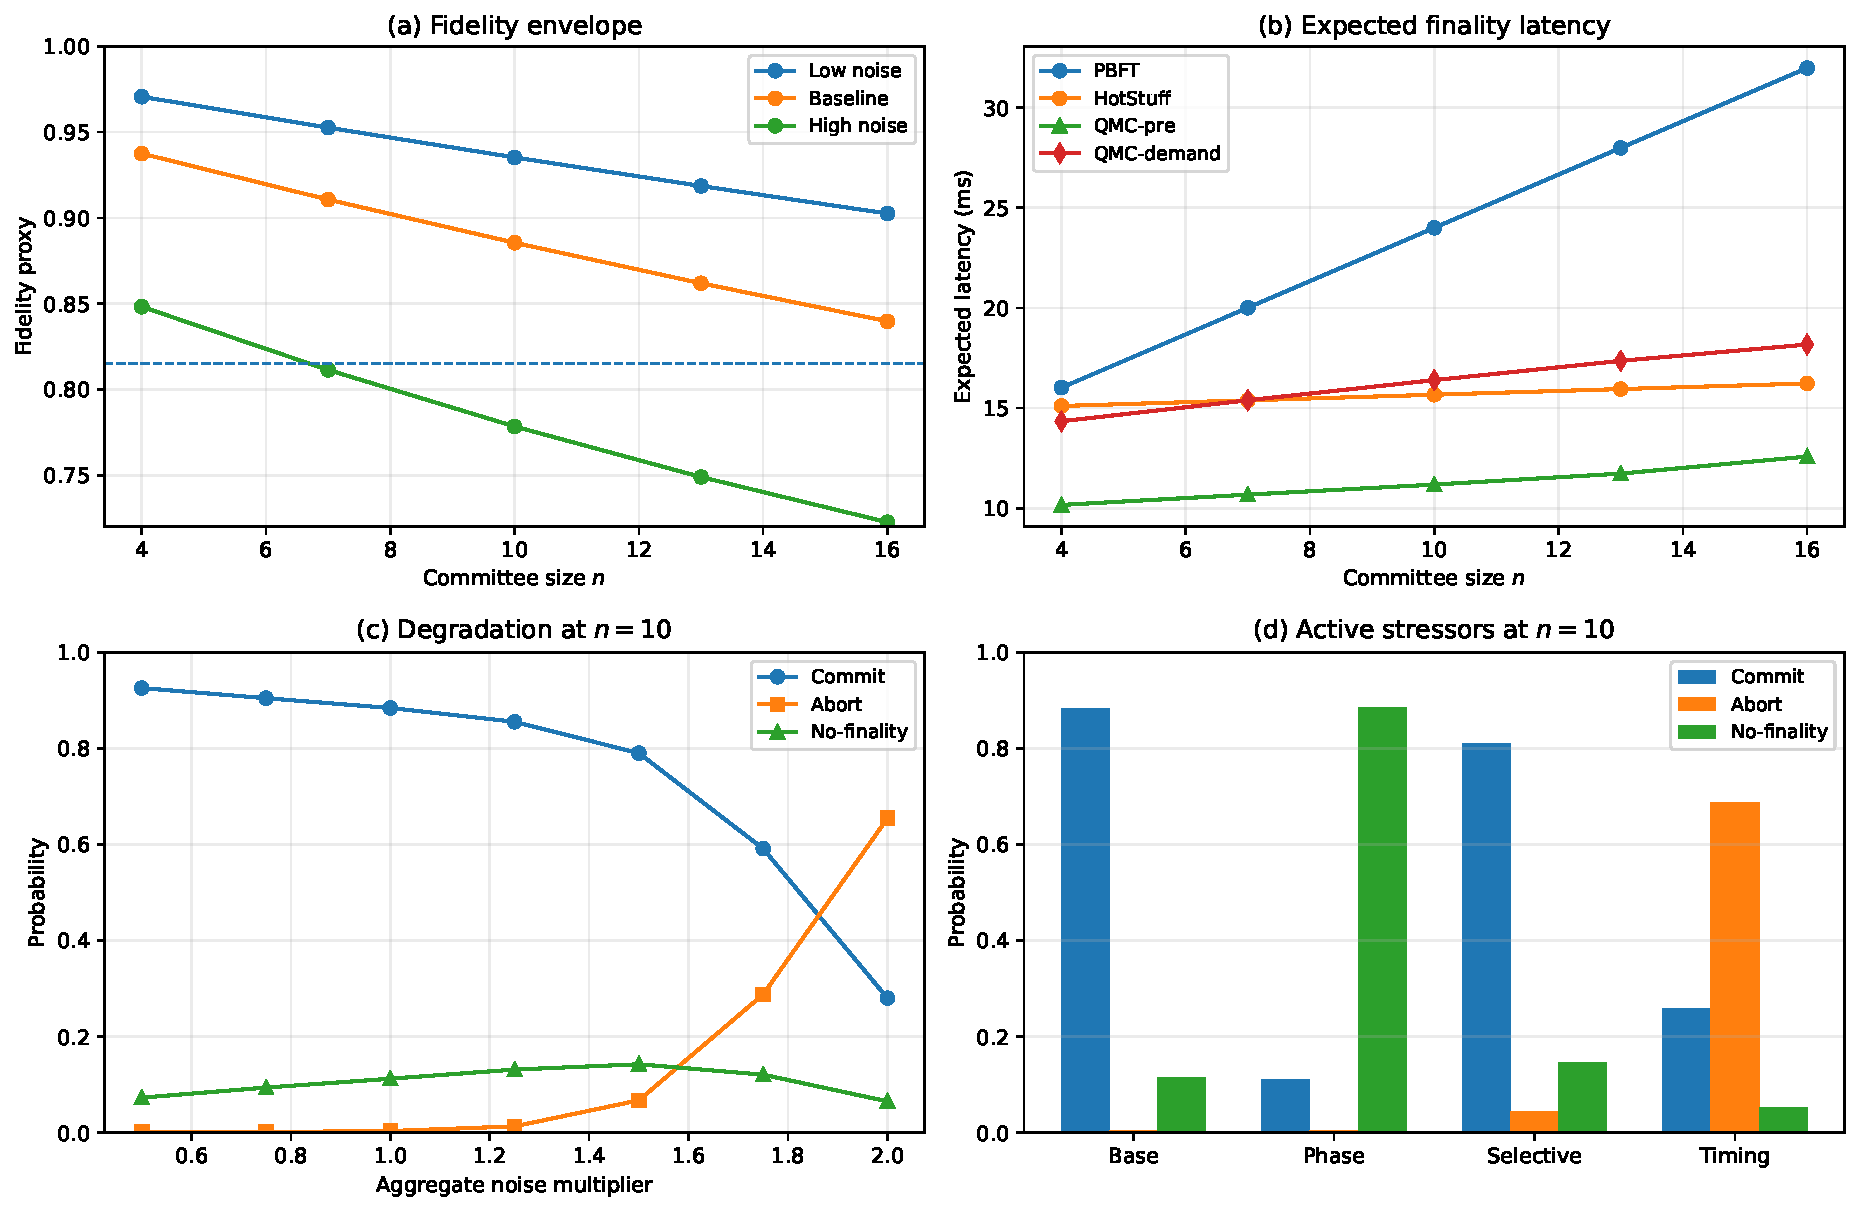
\includegraphics[width=0.98\textwidth]{fig2_quantitative.pdf}
\caption{Quantitative behavior of QMC. (a) Fidelity envelope for three noise regimes. (b) Expected post-certification finality-interval latency for PBFT, HotStuff, QMC with pre-provisioned resource, and QMC with on-demand provisioning. (c) Evolution of the probabilities of \textit{commit}, \textit{abort}, and \textit{no-finality} at $n=10$ as aggregate noise increases. (d) Output distribution under baseline conditions and three active stressors.}
\label{fig:quantitative}
\end{figure*}

\subsection{When does QMC lose to HotStuff?}
Figure~\ref{fig:maps}(a) summarizes fast-path credibility as a joint function of committee size and aggregate noise. The $0.90$ contour is concentrated roughly in the region $n \leq 9$ under baseline noise, while the $0.75$ contour extends to somewhat larger committees under moderate degradation. This makes the intended scope explicit: QMC is not a general solution for large committees.

Figure~\ref{fig:maps}(b) shows how much additional provisioning delay the quantum plan can tolerate before losing its advantage over HotStuff. If extra provisioning delay stays below approximately $5$ ms, QMC still preserves a conditional advantage for small committees; as the committee grows, that tolerance drops rapidly. A compact managerial reading is
\begin{equation}
\lambda\bigl(T_{HS}(n)-\mathbb{E}[T_{QMC}(n,\theta)]\bigr) \geq C_Q,
\label{eq:breakeven}
\end{equation}
where $\lambda$ is the value assigned to each millisecond saved and $C_Q$ is the operational premium of maintaining the quantum plane. Equation~\eqref{eq:breakeven} is not a deep formal result; it is a deployment ruler for deciding when the fast path deserves to exist. Engineering interpretation: the negative result is part of the contribution, because it makes the regime boundary explicit rather than implicit.

\begin{figure*}[!t]
\centering
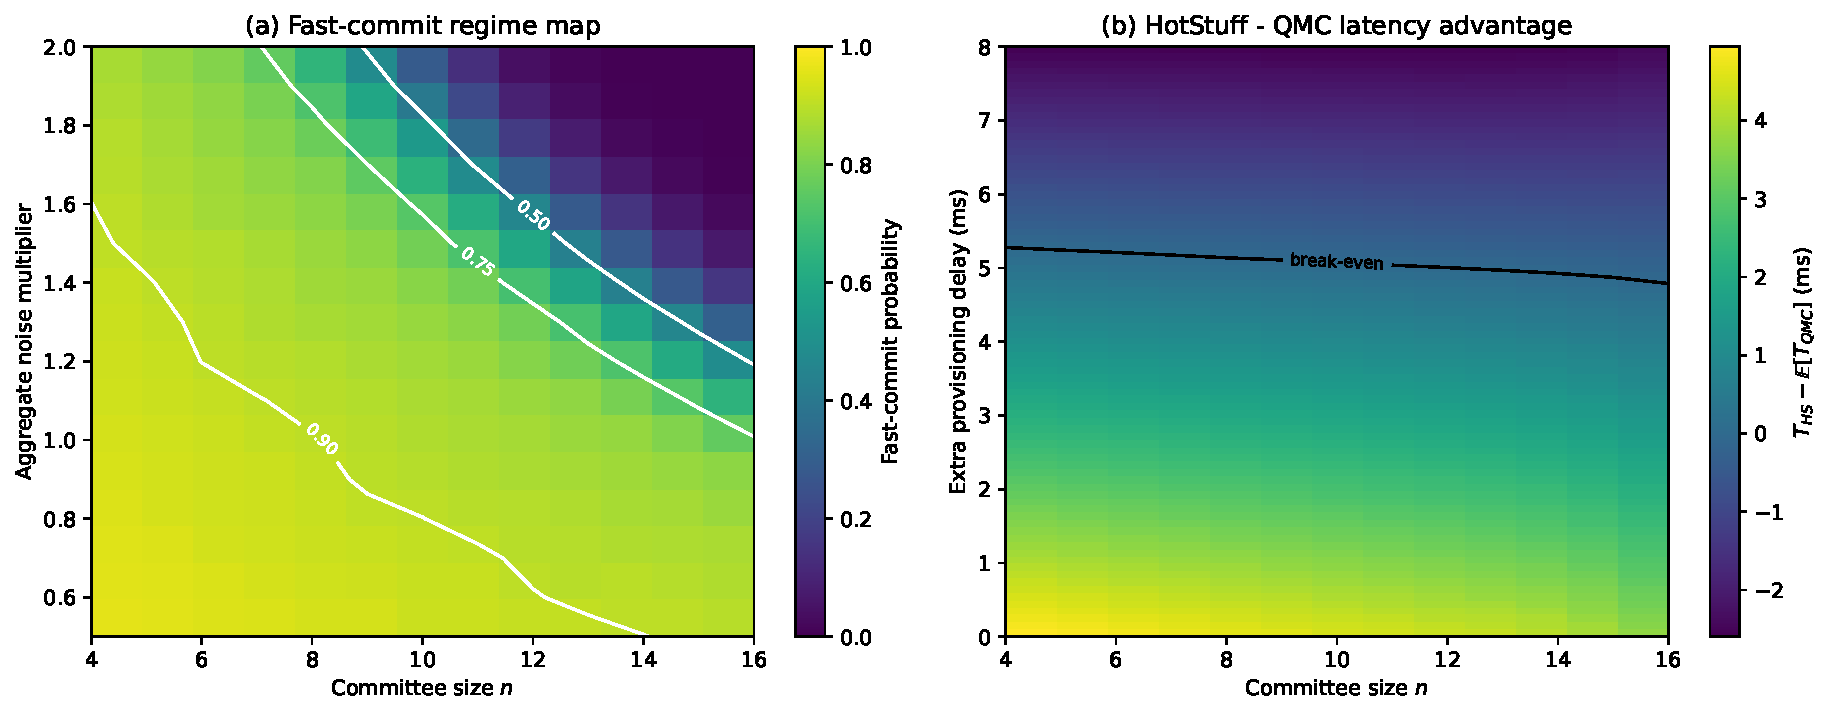
\includegraphics[width=0.98\textwidth]{fig3_regime_maps.pdf}
\caption{Deployment-oriented regime maps for the post-certification finality interval. (a) Fast-commit probability as a joint function of committee size and aggregate noise multiplier. (b) Latency advantage $T_{HS}-\mathbb{E}[T_{QMC}]$ when extra provisioning delay is added to the quantum service plane.}
\label{fig:maps}
\end{figure*}

\subsection{When is a single retry worthwhile?}
Table~\ref{tab:retry} translates~\eqref{eq:retry} into an engineering rule. Under light and medium noise, one retry after \textit{no-finality} still improves fast-commit probability materially. Under heavy noise, most probability mass has already moved to \textit{abort}; insisting on the quantum path adds little value and only increases delay.

The univariate sensitivity analysis of Figure~\ref{fig:sensitivity} supports the same interpretation. At $n=10$, fast-commit probability is highly sensitive to the acceptance threshold $F_{\min}$ and to timing jitter $\sigma_t$, but comparatively stable with respect to estimator uncertainty $\sigma_F$ within the studied range. In other words, synchronization discipline and acceptance policy matter more than marginally refining an estimator that is already operating inside a controlled regime. Engineering interpretation: retry is an engineering convenience, not a new protocol guarantee, and becomes unhelpful once probability mass has already shifted toward abort.

\begin{table}[!t]
\caption{Single-retry policy at $n=10$.}
\label{tab:retry}
\centering
\footnotesize
\renewcommand{\arraystretch}{1.14}
\begin{tabular}{cccc}
\toprule
\textbf{Noise} & $p_c$ & $p_n$ & $p_c^{(1R)}$ \\
\midrule
$1.0\times$ & $0.882$ & $0.114$ & $0.983$ \\
$1.5\times$ & $0.787$ & $0.143$ & $0.899$ \\
$2.0\times$ & $0.280$ & $0.065$ & $0.299$ \\
\bottomrule
\end{tabular}
\end{table}

\begin{figure*}[!t]
\centering
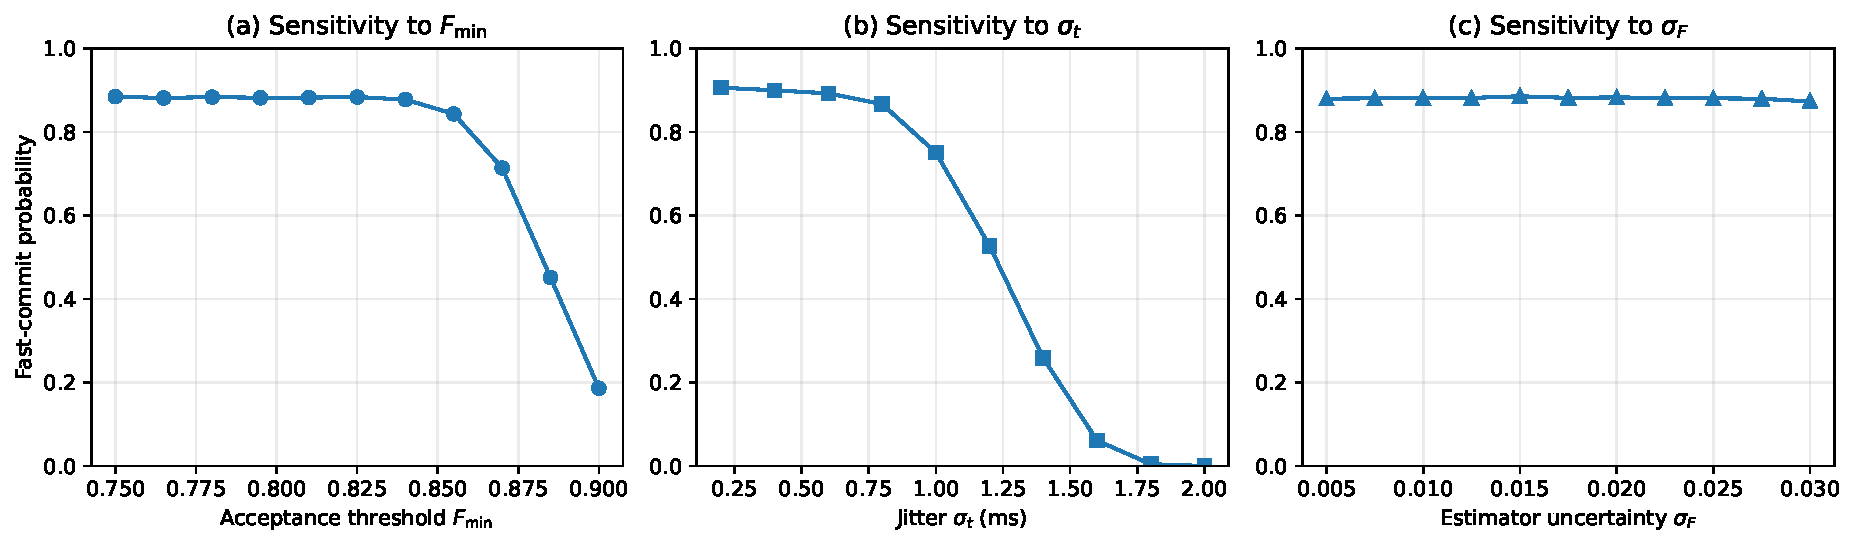
\includegraphics[width=0.98\textwidth]{fig4_sensitivity.pdf}
\caption{Univariate sensitivity of post-certification fast-commit probability at $n=10$: (a) sensitivity to the acceptance threshold $F_{\min}$; (b) sensitivity to timing jitter $\sigma_t$; and (c) sensitivity to estimator uncertainty $\sigma_F$.}
\label{fig:sensitivity}
\end{figure*}

\section{Deployment Guidance, Negative Result, and Limitations}
\label{sec:limits}
The results support selective enablement rather than blanket adoption. QMC should be considered only when (i) the committee is small or medium; (ii) membership is relatively stable; (iii) verified multipartite resources are available, preferably pre-positioned; (iv) the control plane offers strong timing discipline; (v) the ledger already has an always-live classical fallback; and (vi) the application assigns measurable value to a few milliseconds saved during the post-certification finality interval.

The acceptance boundary is operational, not rhetorical. If transcript service p95 latency approaches the $4$--$5$ ms break-even margin, if the fast path is invoked often enough to create sustained queueing, or if replicated transcript dissemination is required in every round, the quantum path should be disabled even if the underlying resource occasionally satisfies the fidelity predicate. The architecture is designed to make that disabling decision safe: a rejected QMC round is an availability loss for the fast path, not a conflicting ledger state.

\subsection{Deployment Zone Summary}
Table~\ref{tab:zones} summarizes the three operational regimes identified by the analysis, with explicit decision criteria. This compact summary is intended to support editorial reading and rapid deployment screening.

\begin{table*}[!t]
\caption{Operational deployment zones: decision summary.}
\label{tab:zones}
\centering
\footnotesize
\renewcommand{\arraystretch}{1.2}
\begin{tabularx}{\textwidth}{p{2.2cm}p{4.5cm}p{4.5cm}Y}
\toprule
\textbf{Zone} & \textbf{Committee \& resource conditions} & \textbf{Transcript \& timing conditions} & \textbf{Recommended policy} \\
\midrule
\textbf{QMC justified} & Small committee ($n \leq 10$); pre-positioned verified GHZ resources; stable membership & Transcript overhead $< 4$ ms; timing jitter $\sigma_t < 1.0$ ms; no sustained queueing ($\rho < 0.7$) & \textbf{Enable QMC}. Use at most one controlled retry after \textit{no-finality}. Monitor transcript latency and fidelity estimates. \\
\midrule
\textbf{QMC marginal} & Medium committee ($10 < n \leq 16$); pre-positioned resources available but with higher orchestration cost; or on-demand resources with low provisioning overhead & Transcript overhead $4$--$5$ ms; timing jitter $1.0$--$1.5$ ms; occasional queueing spikes & \textbf{Enable conditionally}. Use strict monitoring of $F_{\min}$, $\sigma_t$, and transcript p95 latency. Disable automatically if break-even thresholds are crossed. No retry after \textit{no-finality}. \\
\midrule
\textbf{Disable QMC} & Large committee ($n > 16$); on-demand GHZ generation required in most rounds; highly dynamic membership; or no verified multipartite infrastructure & Transcript overhead $> 5$ ms; timing jitter $\sigma_t > 1.5$ ms; sustained queueing ($\rho > 0.85$); or replicated transcript dissemination required per round & \textbf{Keep only classical path}. HotStuff or equivalent classical protocol is the better engineering choice. The quantum fast path provides no meaningful latency advantage and adds operational complexity. \\
\bottomrule
\end{tabularx}
\end{table*}

The boundary between zones is intentionally conservative. The transition from ``justified'' to ``marginal'' occurs near $n=10$ under the baseline surrogate model, and the transition from ``marginal'' to ``disabled'' occurs when extra transcript exhausts the $4$--$5$ ms break-even margin identified in Table~\ref{tab:aggmargin}. The acceptance boundary is operational rather than rhetorical: once transcript latency, queueing, or orchestration overhead consumes the available break-even margin, disabling QMC becomes the correct engineering decision even if the quantum layer remains intermittently usable. These thresholds are not rigid production rules; they are screening criteria derived from the phenomenological analysis.

\subsection{Negative result: when HotStuff remains the better engineering choice}
The analysis also supports a clear negative result within scope: when GHZ generation and distribution must be paid on demand in most rounds, or when timing discipline is weak, HotStuff remains the better engineering choice for the post-certification finality interval. This negative result is important because it supports the interpretation that the methodology was not designed to force a universal quantum advantage.

\subsection{Threats to validity}
\textit{Construct validity.} The physical model is phenomenological; visibility and fidelity are grounded against experimental categories in the literature but are not calibrated to a specific hardware platform.

\textit{External validity.} The conclusions do not extend to permissionless blockchains, highly dynamic committees, or weakly synchronized Internet-scale environments.

\textit{Calibration validity.} The latency models are operational surrogates within the committee range studied; other control stacks or topologies may shift the break-even points.

\textit{Implementation validity.} Maintenance costs, repeaters, multi-tenant scheduling, and quantum CAPEX are excluded from the totals. The independence of repeated attempts in~\eqref{eq:retry} should also be read as an engineering approximation.

\textit{Engineering-validity boundary.} The article provides a regime-based systems evaluation, an analytic transcript break-even screen, and a lightweight transcript-service emulator rather than a hardware-qualified demonstration. Its value is therefore in delimiting the operational envelope of a quantum fast path, not in claiming production readiness of a specific quantum platform.

These validity threats do not weaken the manuscript's internal claim boundary; they define the boundary within which the conclusions should be trusted.

\begin{table*}[!t]
\caption{Deployment-oriented synthesis.}
\label{tab:deployment}
\centering
\scriptsize
\setlength{\tabcolsep}{4pt}
\renewcommand{\arraystretch}{1.14}
\begin{tabularx}{\textwidth}{p{3.0cm}p{2.5cm}p{2.8cm}Y}
\toprule
\textbf{Regime} & \textbf{Expected benefit} & \textbf{Dominant risk} & \textbf{Recommended policy} \\
\midrule
Small committee, pre-positioned GHZ, strong synchronization & Real latency gain over HotStuff & Transcript fault or localized fidelity degradation & Enable QMC with at most one controlled retry after \textit{no-finality}. \\
Medium committee, administrated synchronization, moderate noise & Moderate gain, highly parameter sensitive & Gradual erosion toward \textit{no-finality} and \textit{abort} & Enable QMC only with strict monitoring of $F_{\min}$ and $\sigma_t$. \\
Medium/large committee with on-demand provisioning & Marginal or null advantage & Provisioning delay destroys break-even & Prefer HotStuff as the default engineering choice. \\
Weak timing discipline or strong coordinated misalignment & Almost no sustained gain & Abort-dominant behavior under timing stress & Disable the quantum fast path and keep only classical recovery. \\
\bottomrule
\end{tabularx}
\end{table*}

\section{Conclusion}
\label{sec:conclusion}
This article asked a narrow systems question: whether a quantum-assisted service can shorten the post-certification finality interval of a permissioned ledger without enlarging the ledger's safety surface. The answer provided by the manuscript is conditional but technically disciplined: QMC contributes a ledger-integrated transcript-authenticated fast path, proves safety preservation under standard assumptions, and evaluates bounded operational regimes in which that fast path may or may not be justified.

Within scope, the conditional advantage appears only when committees remain small to medium, multipartite resources are pre-provisioned and verified, timing discipline is strong, and transcript aggregation stays below the break-even envelope identified by the screening analysis. Once transcript delay, queueing, or orchestration overhead grows beyond that envelope, the correct engineering decision is to disable the fast path and rely on mature classical finality.

The paper therefore establishes a conservative protocol architecture and a deployment decision framework, not a production-readiness claim. Its practical contribution is to show how quantum evidence could be made ledger-consumable under a fail-closed systems envelope, and to make explicit the conditions under which that effort should be abandoned in favor of mature classical finality.

\appendices
\section{Optional Composite Metric for Deployment Decisions}
In some deployments, it may be convenient to combine latency and success rate into one composite quantity,
\begin{equation}
\Psi(n,\theta) = \Pr[\mathrm{commit}]\left(T_{HS}(n)-\mathbb{E}[T_{QMC}(n,\theta)]\right).
\label{eq:psi}
\end{equation}
Positive values of $\Psi$ indicate that latency advantage remains meaningful after weighting by the probability of fast commit. The metric does not replace the main analysis, but it can be useful as a deployment-side screening tool.

\begin{thebibliography}{00}

\bibitem{b1} L. Lamport, R. Shostak, and M. Pease, ``The Byzantine generals problem,'' \emph{ACM Trans. Program. Lang. Syst.}, vol. 4, no. 3, pp. 382--401, 1982.

\bibitem{b2} M. Castro and B. Liskov, ``Practical Byzantine fault tolerance,'' in \emph{Proc. 3rd Symp. Operating Systems Design and Implementation}, 1999, pp. 173--186.

\bibitem{b3} E. Buchman, \emph{Tendermint: Byzantine Fault Tolerance in the Age of Blockchains}. M.S. thesis, Univ. Guelph, Guelph, ON, Canada, 2016.

\bibitem{b4} G. G. Gueta \emph{et al.}, ``SBFT: A scalable and decentralized trust infrastructure,'' in \emph{Proc. IEEE/IFIP Int. Conf. Dependable Systems and Networks}, 2019, pp. 568--580.

\bibitem{b5} M. Yin \emph{et al.}, ``HotStuff: BFT consensus with linearity and responsiveness,'' in \emph{Proc. ACM Symp. Principles of Distributed Computing}, 2019, pp. 347--356.

\bibitem{b6} S. Bano \emph{et al.}, ``SoK: Consensus in the age of blockchains,'' in \emph{Proc. 1st ACM Conf. Advances in Financial Technologies}, 2019, pp. 183--198.

\bibitem{b7} M. Fitzi, N. Gisin, and U. Maurer, ``Quantum solution to the Byzantine agreement problem,'' \emph{Phys. Rev. Lett.}, vol. 87, no. 21, Art. no. 217901, 2001.

\bibitem{b8} S. Iblisdir and N. Gisin, ``Byzantine agreement with two quantum-key-distribution setups,'' \emph{Phys. Rev. A}, vol. 70, no. 3, Art. no. 034306, 2004.

\bibitem{b9} S. Gaertner \emph{et al.}, ``Experimental demonstration of a quantum protocol for Byzantine agreement and liar detection,'' \emph{Phys. Rev. Lett.}, vol. 100, no. 7, Art. no. 070504, 2008.

\bibitem{b10} V. Cholvi, ``Quantum Byzantine agreement for any number of dishonest parties,'' \emph{Quantum Inf. Process.}, vol. 21, Art. no. 151, 2022.

\bibitem{b11} Z. Qu \emph{et al.}, ``Quantum detectable Byzantine agreement for distributed data trust management in blockchain,'' \emph{Inf. Sci.}, vol. 637, Art. no. 118909, 2023.

\bibitem{b12} X. Jing \emph{et al.}, ``Experimental quantum Byzantine agreement on a three-user quantum network with integrated photonics,'' \emph{Sci. Adv.}, vol. 10, no. 34, Art. no. eadp2877, 2024.

\bibitem{b13} J. Sousa, A. Bessani, and M. Vukolic, ``A Byzantine fault-tolerant ordering service for the Hyperledger Fabric blockchain platform,'' in \emph{Proc. IEEE/IFIP Int. Conf. Dependable Systems and Networks}, 2018, pp. 51--58.

\bibitem{b14} E. Androulaki \emph{et al.}, ``Hyperledger Fabric: A distributed operating system for permissioned blockchains,'' in \emph{Proc. 13th EuroSys Conf.}, 2018, Art. no. 30.

\bibitem{b15} C. Stathakopoulou, T. David, M. Pavlovic, and M. Vukolic, ``Mir-BFT: High-throughput robust BFT for decentralized networks,'' \emph{CoRR}, abs/1906.05552, 2019.

\bibitem{b16} R. Kotla, L. Alvisi, M. Dahlin, A. Clement, and E. Wong, ``Zyzzyva: Speculative Byzantine fault tolerance,'' in \emph{Proc. ACM SIGOPS Symp. Operating Systems Principles}, 2007, pp. 45--58.

\bibitem{b17} X. Sun, P. Kulicki, and M. Sopek, ``Multi-party quantum Byzantine agreement without entanglement,'' \emph{Entropy}, vol. 22, no. 10, Art. no. 1152, 2020.

\bibitem{b18} T. Andronikos and A. Sirokofskich, ``A quantum detectable Byzantine agreement protocol using only EPR pairs,'' \emph{Appl. Sci.}, vol. 13, no. 14, Art. no. 8405, 2023.

\bibitem{b19} Y.-G. Han, Z.-H. Liu, H. Zhu, and M. Hayashi, ``Optimal verification of the Bell state and Greenberger-Horne-Zeilinger states in untrusted quantum networks,'' \emph{npj Quantum Inf.}, vol. 7, Art. no. 150, 2021.

\bibitem{b20} Z. Bao \emph{et al.}, ``Creating and controlling global Greenberger-Horne-Zeilinger entanglement on quantum processors,'' \emph{Nat. Commun.}, vol. 15, Art. no. 8823, 2024.

\bibitem{b21} W.-T. Kao \emph{et al.}, ``Scalable determination of multipartite entanglement in quantum networks,'' \emph{npj Quantum Inf.}, vol. 10, Art. no. 73, 2024.

\bibitem{b22} L. Oleynik, J. U. Rehman, S. Koudia, and S. Chatzinotas, ``Entanglement distribution in lossy quantum networks,'' \emph{Sci. Rep.}, vol. 15, Art. no. 29778, 2025.

\bibitem{b23} N. H. Valencia \emph{et al.}, ``A large-scale reconfigurable multiplexed quantum photonic network,'' \emph{Nat. Photon.}, vol. 20, pp. 202--207, 2026.

\bibitem{b24} C. Dwork, N. Lynch, and L. Stockmeyer, ``Consensus in the presence of partial synchrony,'' \emph{J. ACM}, vol. 35, no. 2, pp. 288--323, 1988.

\bibitem{b25} G. Bracha, ``Asynchronous Byzantine agreement protocols,'' \emph{Inf. Comput.}, vol. 75, no. 2, pp. 130--143, 1987.

\end{thebibliography}

\begin{IEEEbiographynophoto}{Davy Mateus Nzamba}
Davy Mateus Nzamba is with the Departamento Academico de Eletrotecnica, Universidade Tecnologica Federal do Parana (UTFPR), Curitiba, Parana, Brazil. His current research interests include permissioned blockchains, Byzantine fault tolerance, distributed systems, and quantum-assisted networked systems.
\end{IEEEbiographynophoto}

\begin{IEEEbiographynophoto}{Ricardo Fernandes da Silva}
Ricardo Fernandes da Silva is with the Departamento Academico de Fisica, Universidade Tecnologica Federal do Parana (UTFPR), Curitiba, Parana, Brazil. His current research interests include quantum information, quantum networks, complex systems, and interdisciplinary applications of physics to distributed technologies.
\end{IEEEbiographynophoto}

\EOD
\end{document}
